\documentclass[12pt]{article}
\usepackage[utf8]{inputenc}

\usepackage{ragged2e}
\usepackage{graphicx}
\usepackage{wrapfig}


%\usepackage[margin=1.2in]{geometry}

\title{\huge ECAL DCS Beginners Manual}
\author{authors}
\date{\today}

\begin{document}

\maketitle

\newpage
\tableofcontents
\newpage


\section{Introduction}

\justifying
Cosa serve questo manuale? Serve a spiegare con immagini e spiegazioni le informazioni base per saper usare il dcs dell'ecal e capire cosa sono le diverse parti e come si usano. Le immagini allegate sono prese da una macchina virtuale, ma è come se fosse il vero dcs panel.
Il manuale è per i beginner e vuole introdurre i concetti principali e le cose principali da sapere per un operator on call dell'ecal dcs.
 
\newpage
\section{First steps - How to access to the DCS}
 Chiedi a raul che ne pensa, se conviene fare una sezione in cui si spiega come si accede alla macchina virtuale e poi dire come si accede a cms
Qui scriverei come si accede al dcs. Scriverei come si fa dicendo che per ogni sistema operativo ho un coso diverso, per esempio io ho rammina, poi da lì devo accedere a cernts.cern.ch e da lì da un'altra parte? (che non è dove accedo io perchè quella è la macchina virtuale). Quindi io posso fa le foto del mio e lascio spazio per dove dovrebbe essere la parte vera. Poi scrivo anche come modificare le preferenza per avere schermo grande, senno non si vede (però solo con ramnina)

\section{The ECAL DCS panels}
%Una volta entrato nel DCS, la prima schermata che ci si trova davanti è quella in figura 1.
Once entered in the DCS, the first screen that can be seen in the one in Fig. \ref{fig:mainpanel}. The first thing to do is to log in with your personal account, with a right click on "NO USER", written in the upper right corner of the panel, as suggested bu the red arrow in \ref{fig:mainpanel}, or clicking on the close key.  

\begin{figure}[!h]
	\centering
	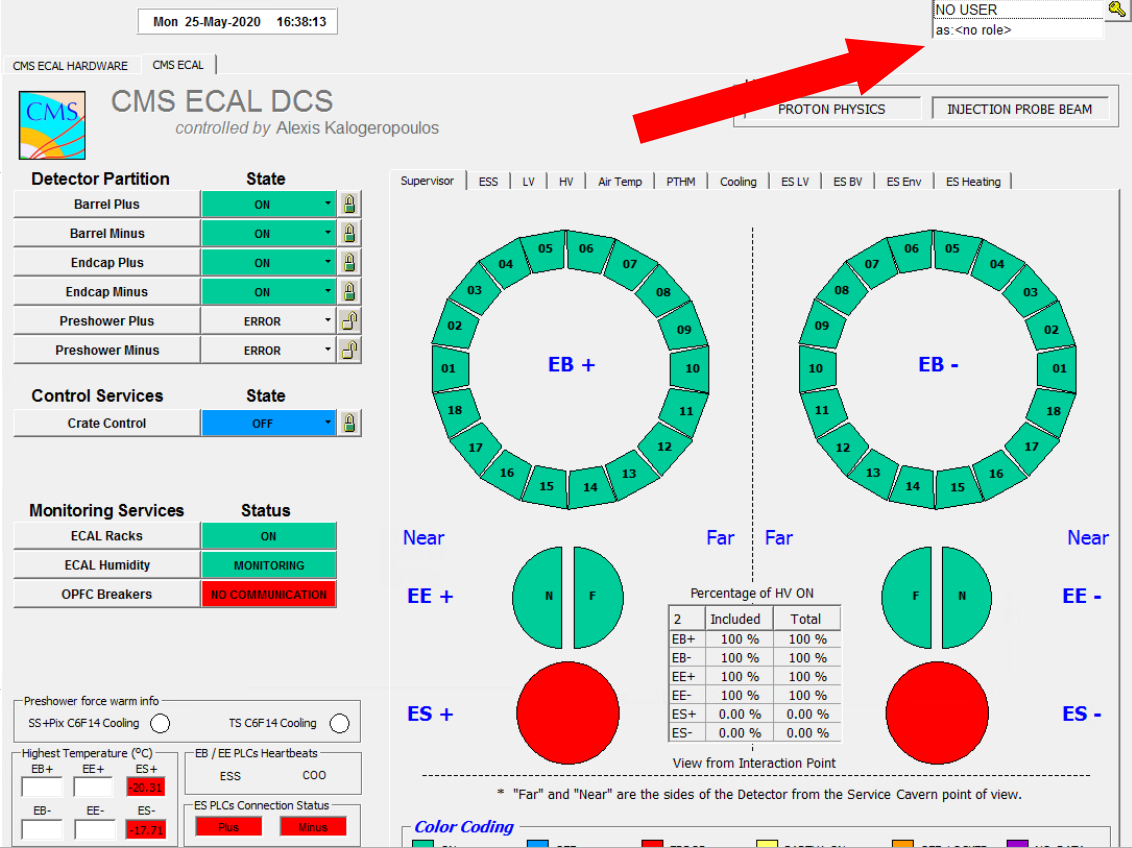
\includegraphics[width=1\textwidth]{Pics/Principal_witharrow}
	\caption{Principal window of the DCS. The red arrow indicates where to click to login, as explained in the text. }
	\label{fig:mainpanel}
\end{figure}

Consequently the window showed in Fig. \ref{fig:access} on the left is going to appear. There you should insert your username and your personal password. If everything is correct, there will not be any error and the right corner of the DCS panel will appear as in Fig. \ref{fig:access} on the right, with your username. The last action to do to complete the login is to choose your role. You can right click where indicated by the red arrow in Fig. \ref{fig:access} on the right and choose your role, that most probably is "ECAL\_Supervisor\_Operator"

\begin{figure}[!h]
	\centering
	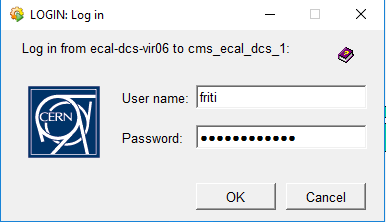
\includegraphics[width=0.4\textwidth]{Pics/login1}
	\quad
	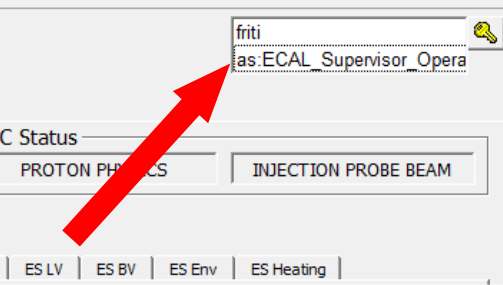
\includegraphics[width=0.4\textwidth]{Pics/login2_witharrow}
	\caption{\textit{On the left.} The log in window that pops up when clicking on the key on the main panel. You should insert your username and password to log in. \textit{On the right.} After the log in, your username will show in the main panel. The red arrow indicated where to right click to change your role.}
	\label{fig:access}
\end{figure}
\subsection{Supervisor panel}
The principal panel in the one that can be seen as soon as you eneter in the DCS. In Fig \ref{fig:principalpanel_withnumbers} three important areas of the main panel have been highlighted, and they will be explained in the following. 

\begin{figure}[!h]
	\centering
	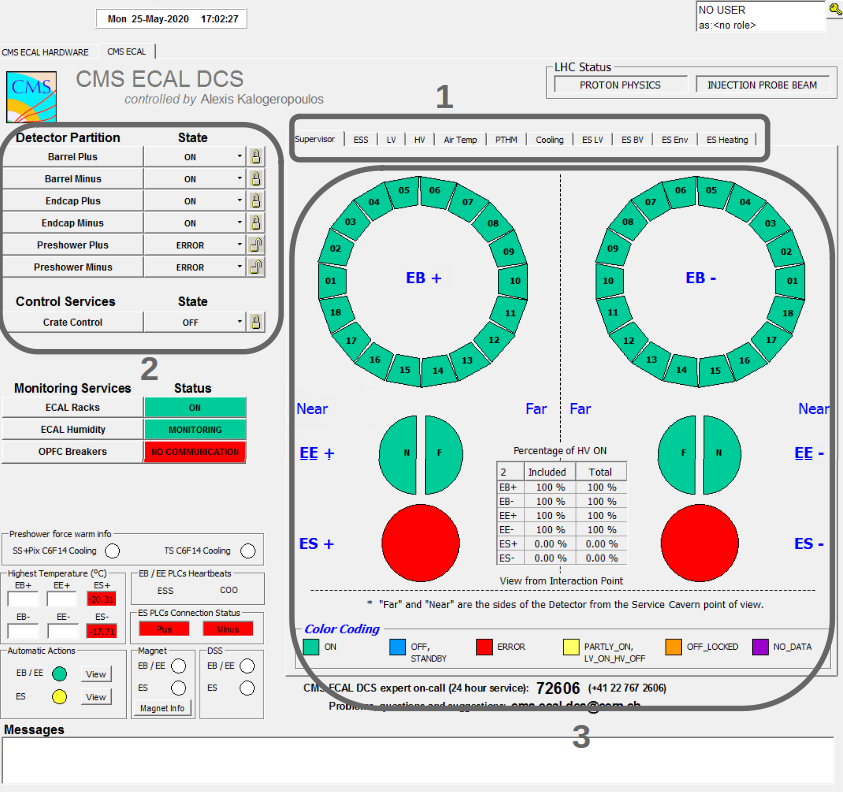
\includegraphics[width=1\textwidth]{Pics/principalpanel_withnumbers.png}
	\caption{Main panel of the DCS. Three important areas of the panel have been circled and are explained in the text.}
	\label{fig:principalpanel_withnumbers}
\end{figure}


\begin{enumerate}
	\item The first area includes different tabs. Each tab represents a different ECAl subsystem, which status must be monitored. The first, the "Supervisor", is the main panel, that is a summary of all the others. The details of each panel will be deeply explained in the following sections (\ref{sec:ESS} - \ref{sec:Preshower}).
	\item In this area it is possible to carry out a check of the ECAL status considering its different partitions. Each partition has a "tree" composition, because it is possible to access all the different subparts that compose the partitions. This important feature, that will be explained better in Section \ref{sec:tree}, is very useful because, if there is a problem, it is possible to find exactly which component has this problem. 
	\item The third area is the summary of the status of each partition of the ECAL. The graphical representation is very useful to have a fast and easily readeble summary of the ECAL status. \\
	In the upper part there are the Supermodules of the ECAL Barrel (EB), plus and minus. Below these there is the representation of the ECAL Endcap (EE), divided into Near (N) and Far (F), and of the Preshower (ES). The latter is attached to the Endcaps. \\
	The legend on the bottom helps in undertanding the meaning of each color, which represents a different status of the calorimeter:
	\begin{itemize}
		\item ON $\rightarrow$ when the partition is working;
		\item OFF, STANDBY $\rightarrow$ when the partition is off or in standby;
		\item ERROR $\rightarrow$ the partition with this color has an error;
		\item PARTLY\_ON, LV\_ON\_HV\_OFF $\rightarrow$ the high voltage is OFF and the low voltage is ON;
		\item OFF\_LOCKED $\rightarrow$ the ECAL is OFF in a safety mode;
		\item NO\_DATA $\rightarrow$ the ECAL is not acquiring data.
	\end{itemize}

From Fig. \ref{fig:principalpanel_withnumbers} it is possible to see that everything in in status ON, except for the ES, which is in state ERROR. As mentioned in the Introduction, all the screens of the DCS showed in this Manual are taken from a Virtual Machine. In this particular virtual machine the ES components were not working, but usually, in the actual DCS, there should be no errors. 
\end{enumerate}
\subsection{ESS Panel}
\label{sec:ESS}
\begin{figure}[!h]
	\centering
	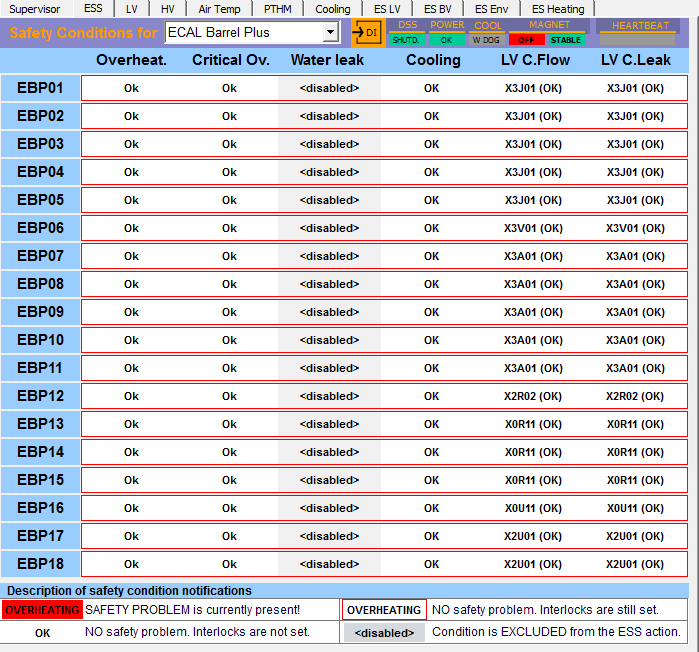
\includegraphics[width=1\textwidth]{Pics/ESS_panel.png}
	\caption{ESS Panel}
	
\end{figure}

\subsection{Low Voltage (LV) and High Voltage Panels}
These two panels can be accesed clicking in the tabs LV and HV respectively, showed in Fig. \ref{fig:principalpanel_withnumbers} in the first circled area. As can be checked in Fig \ref{fig:LVHV}, they are very similar to the principal panel, the \textit{Supervisor} tab. The difference is that the principal panel shows a summary of the status of the ECAl and the Preshower, while here there is only information about LV (and HV) in the ECAL. Indeed there is no information about the ES, which can be found in other tabs (see section \ref{sec:Preshower}).

\begin{figure}[!h]
	\centering
	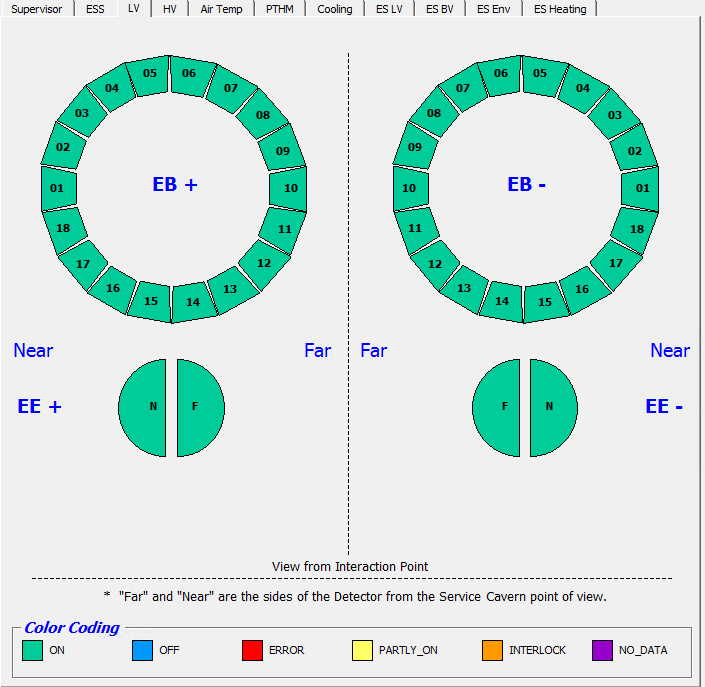
\includegraphics[width=0.48\textwidth]{Pics/LV_panel.png}
	\quad 
		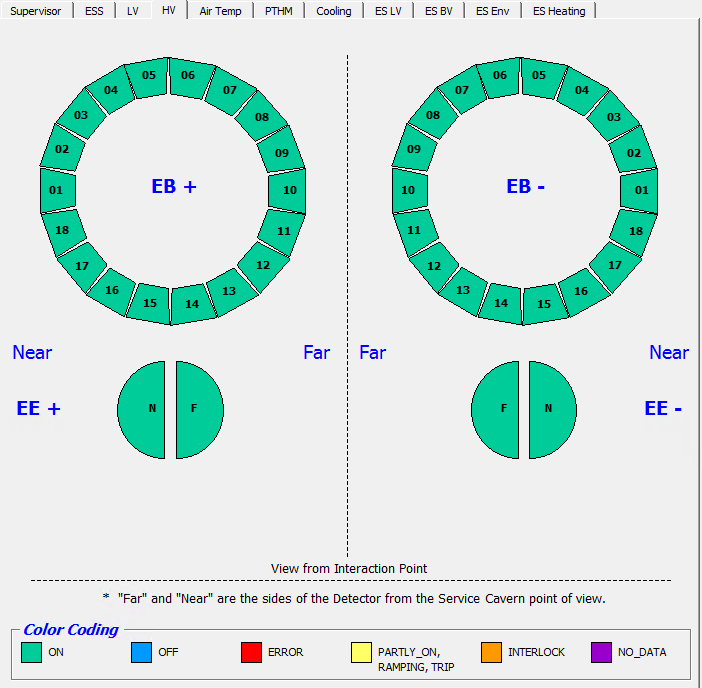
\includegraphics[width=0.48\textwidth]{Pics/HV_panel.png}
	\caption{\textit{On the left.} Low Voltage panel. \textit{On the right.} High Voltage panel.\\  They show the status of the LV (HV) in the ECAL Barrel and in the ECAL Endcap, using the same color legend as in the Supervisor panel. }
	\label{fig:LVHV}
\end{figure}

Let's now consider the case in which the HV in the positive Barrel is OFF. In this situation is important to undertand the role of each tab to really undertand what is happening. In the Supervisor panel (Fig. \ref{fig:HVOFF_main}), where we have a summary of all the ECAl situation, there is the EB+ in the yellow status, which means LV\_ON\_HV\_OFF.

\begin{figure}[!h]
	\centering
	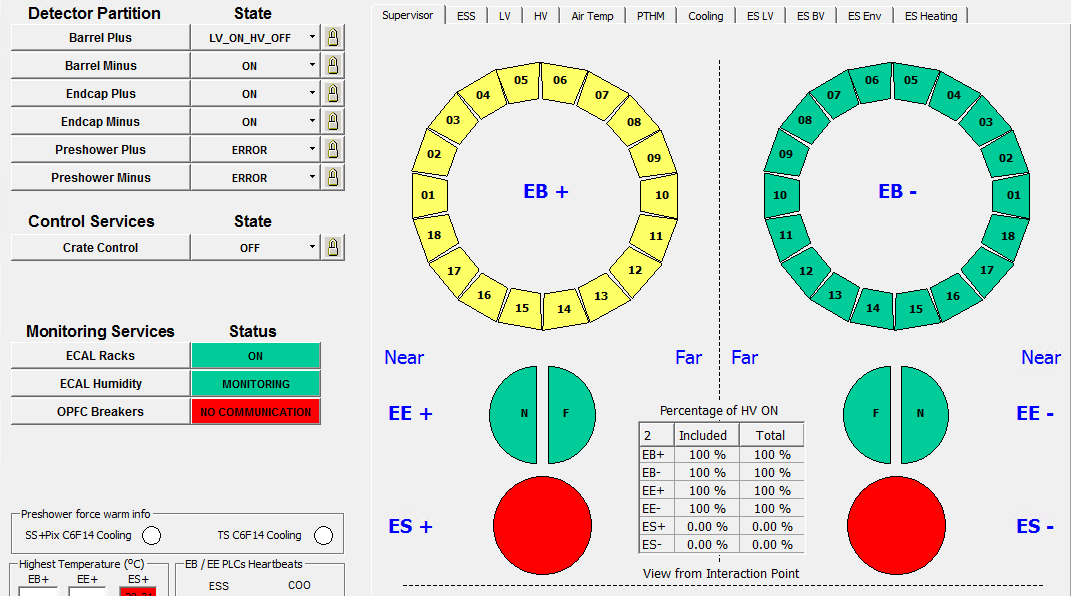
\includegraphics[width=0.9\textwidth]{Pics/Mainpanel_HVOFF.png}
	\caption{This is the Supervisor panel of the DCS with the EB+ with the HV OFF. This can be seen by the graphical representation of the ECA, in which the EB+ is yellow, which means PARTLY\_ON, and in the left side of the window, where it is explicitly written, in correspondence of "Barrel Plus", that it is in the status of LV\_ON\_HV\_OFF.}
	\label{HVOFF_main}
\end{figure}

The status can be also checked in the LV and HV panels, as shown in Fig. \ref{fig:HVOFF_LVHV}. On the left the LV panel is shown, and the status is all ON, while the figure n the right, that represents the HV panel, shows that the EB+ is OFF.

\begin{figure}[!h]
	\centering
	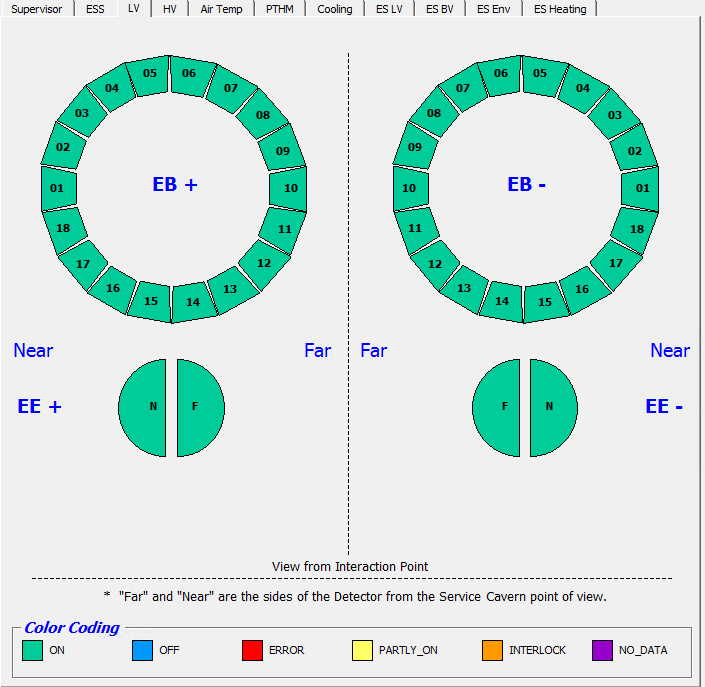
\includegraphics[width=0.48\textwidth]{Pics/LV_panel.png}
	\quad 
	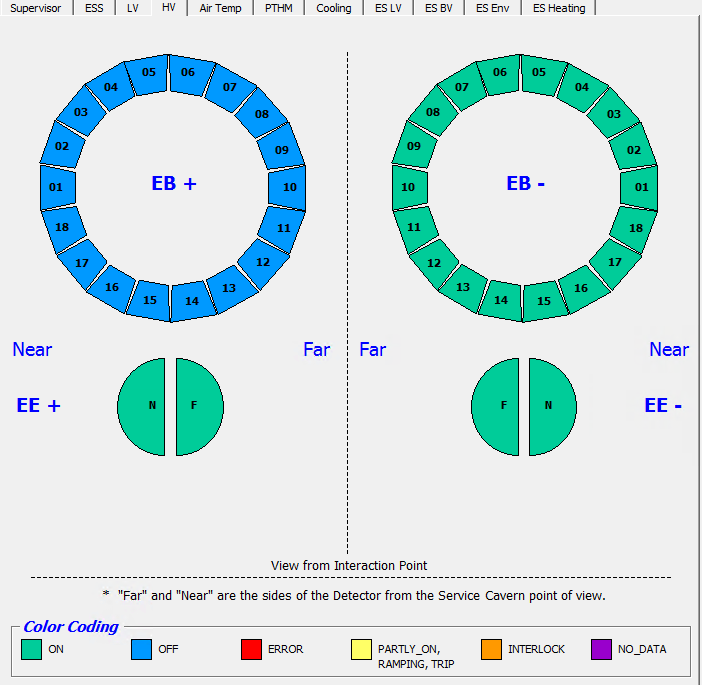
\includegraphics[width=0.48\textwidth]{Pics/HV_OFF.png}
	\caption{These are the screens of the ECAL DCS panels LV and HV in the situation described in Fig. \ref{fig:HVOFF_LVHV}. \textit{On the left.} The LV panel, in which everything is ON. \textit{On the right.} The HV panel, in which the EB+ barrel has the OFF status. }
	\label{fig:HVOFF_LVHV}
	

\end{figure}

In conclusion, depending on the tab that we are visiting, it is possible to access to a detailed or summary information. 


\subsection{AirTemp, PTHM, Cooling Panels}
The parameters of Air Temperature (AirTemp), of Pressure Temperature Humidity Monitoring (PTHM) and Cooling are shown in the respective tabs. This information comes from the Safety System ECAL. These are only control parameters, they can not be modified, but they need to be checked to be sure that everything is working. The screens in Fig. \ref{fig:AirPTHM} and Fig. \ref{fig:Cooling} show how these panels appear. Again they are very similar to the principal panel. The PTHM and Cooling panels also show the temperature of the water, in place of the violet boxes, which represent the NO\_DATA state. The figures here reported are taken from a Virtual Machine, so the Safety System outputs are not connected, as it is possible to be seen in Fig. \ref{fig:Cooling}.
\begin{figure}[!h]
	\centering
	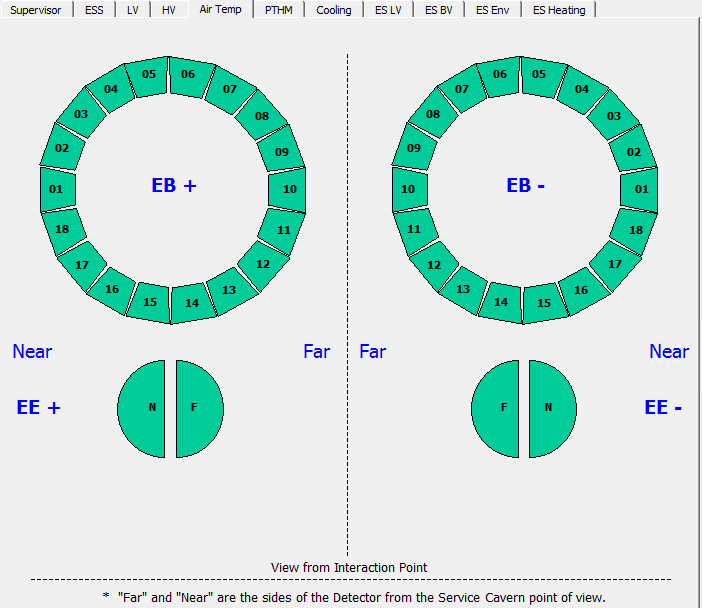
\includegraphics[width=0.48\textwidth]{Pics/AirTemp.png}
	\quad 
	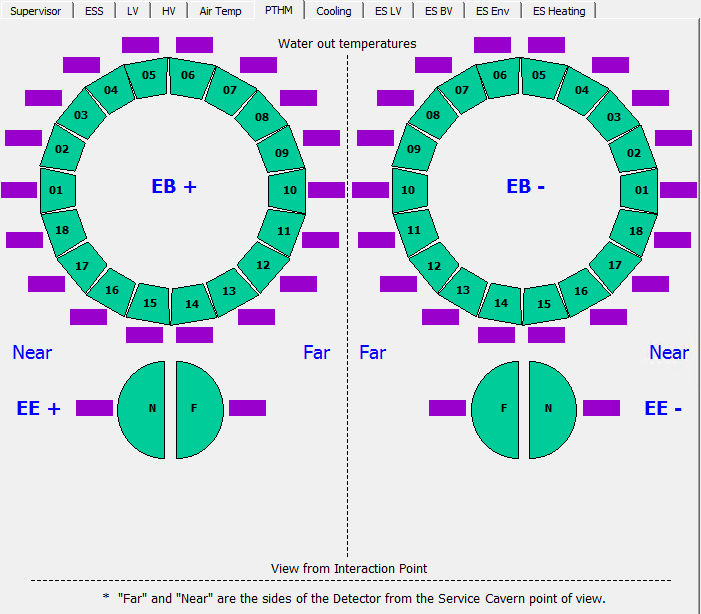
\includegraphics[width=0.48\textwidth]{Pics/PTMH.png}
	\caption{\textit{On the left.} The AirTemp panel. \textit{On the right.} The PTMH panel. The peculiarity here is the information about the water temperature, in place of the violet boxes, that here is not showed because the virtual machine from which the pictures are taken is not connected to any Safety System.}
	\label{fig:AirPTHM}
\end{figure}

\begin{figure}[!h]
	\centering
	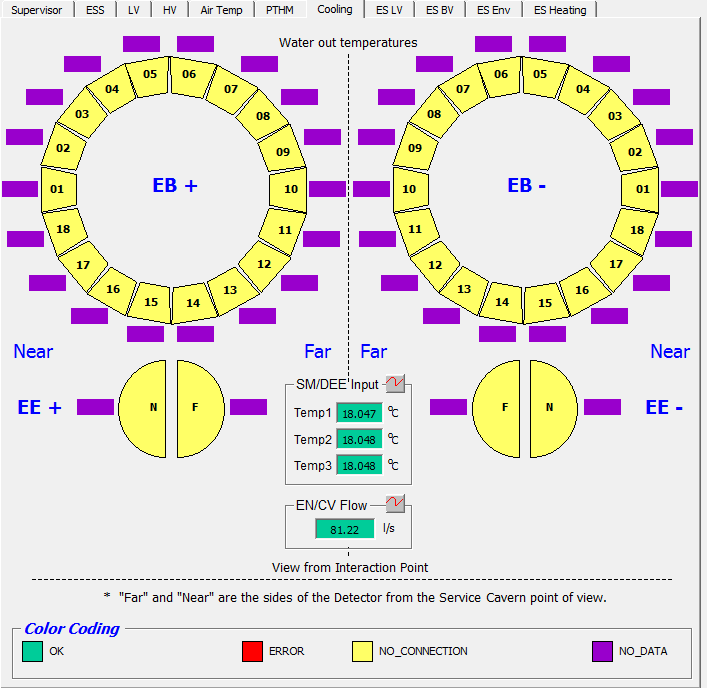
\includegraphics[width=0.48\textwidth]{Pics/Cooling.png}
	\caption{The Cooling Panel. }
	\label{fig:Cooling}
	
	
\end{figure}


\subsection{Preshower Panels}
\label{sec:Preshower}

\begin{figure}[!h]
	\centering
	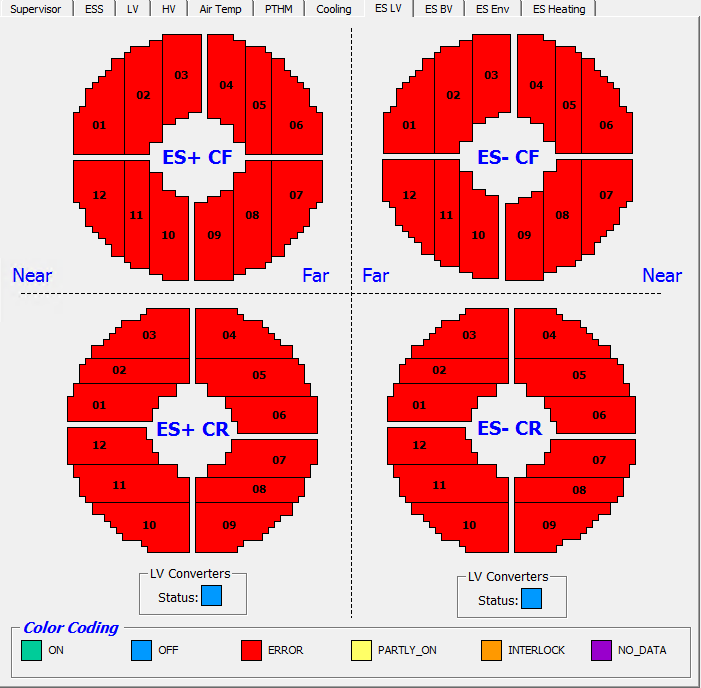
\includegraphics[width=0.48\textwidth]{Pics/ESLV.png}
	\quad 
	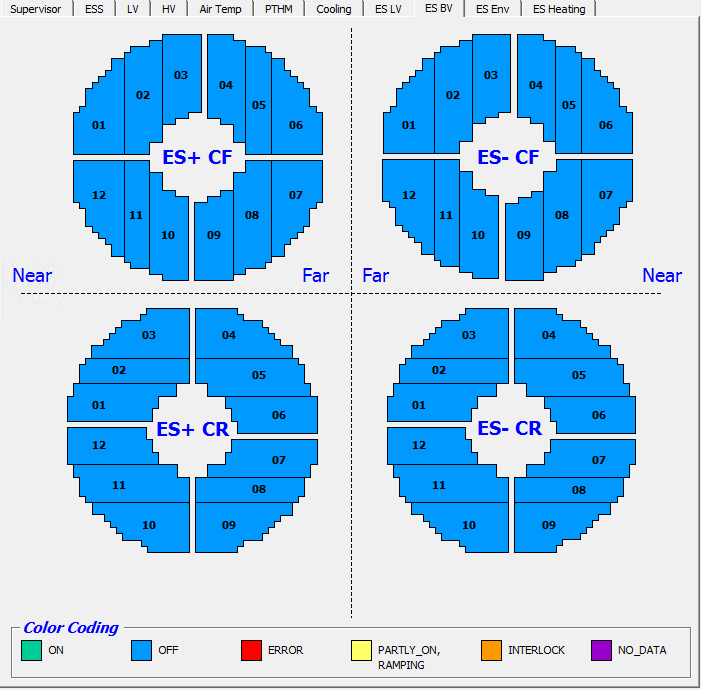
\includegraphics[width=0.48\textwidth]{Pics/ESBV.png}
	\caption{\textit{On the left.} The AirTemp panel. \textit{On the right.} The PTMH panel. The peculiarity here is the information about the water temperature, in place of the violet boxes, that here is not showed because the virtual machine from which the pictures are taken is not connected to any Safety System.}
	\label{fig:AirPTHM}
\end{figure}

\begin{figure}[!h]
	\centering
	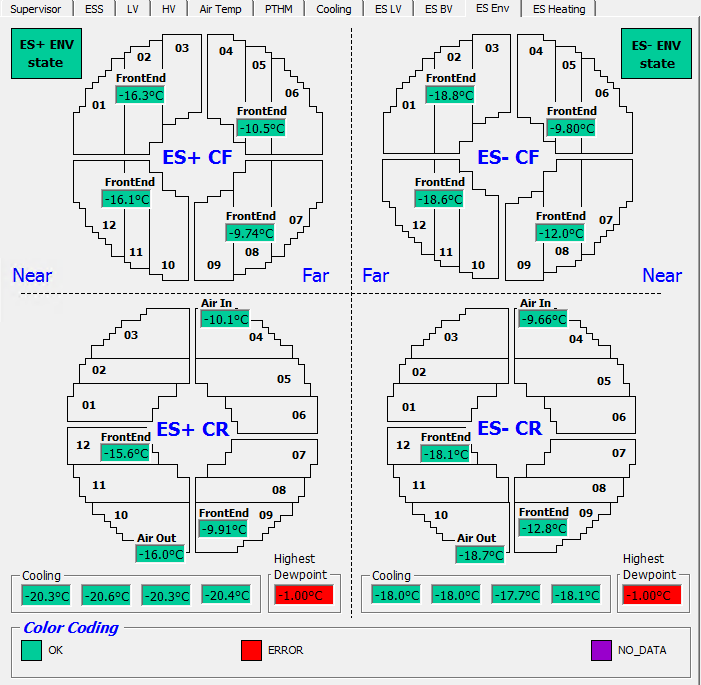
\includegraphics[width=0.48\textwidth]{Pics/ESEnv.png}
	\quad 
	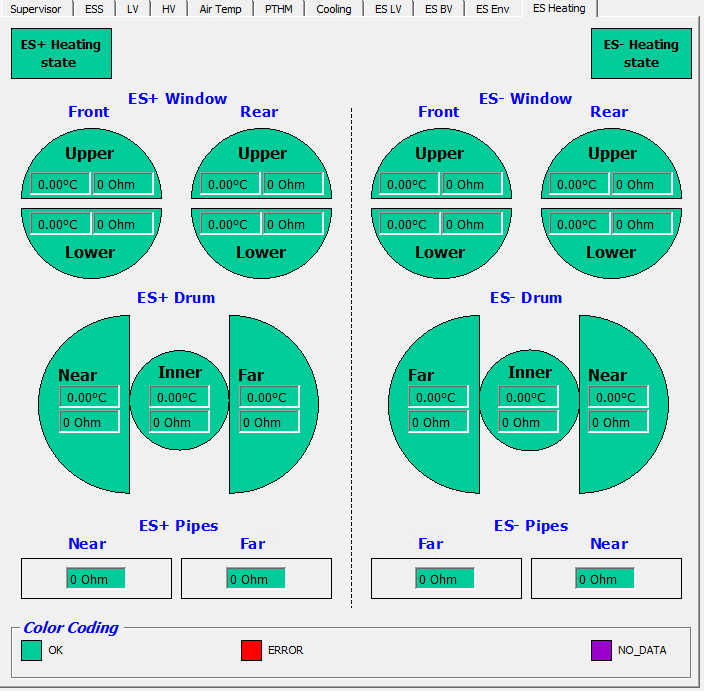
\includegraphics[width=0.48\textwidth]{Pics/ESHeat.png}
	\caption{\textit{On the left.} The AirTemp panel. \textit{On the right.} The PTMH panel. The peculiarity here is the information about the water temperature, in place of the violet boxes, that here is not showed because the virtual machine from which the pictures are taken is not connected to any Safety System.}
	\label{fig:AirPTHM}
\end{figure}
All the other panels are dedicated to the Preshower.
Heating ayer tra preshower e endcap perche hanno temperature di cooling molto divers, preshower 18 gradi centigradi
\section{Detector Partition}
The second area showed in Fig. \ref{fig:principalpanel_withnumbers}, represents 
sto coso è fatto a tree, se clicco su uno, vado sotto e trovo le altre componenti e così via, fai vedere tutte foto.
se per esempio ho un errore su una componente, posso risalire il tree finche non trovo esattamente dove si trova, cosi ho tutto aotto controllo. 
metti un errore e fai foto progressive
\end{document}
